Das Ergebnis der Umsetzung zur Schaffung einer Schnittstelle mit Hilfe eines Signatur-Tablets und der Sage Office Line ist auf den Abbildungen zu sehen. Die Schnittstelle dient zur Erfassung einer digitalen Signatur. Die Verbindung zwischen dem Signatur-Tablet und dem Computer, auf dem die Sage Office Line läuft, wird mit Hilfe eines USB- oder COM-Port realisiert. Die Abbildnung 7 zeigt die Hauptansicht der Sage Office Line. Die roten Markierungen am linken Rand zeigen die Bereiche in dem die Schnittstelle zur Erfassung von digitalen Signaturen integriert wurde. Auf der Abbildung 8 sieht man den Arbeitsablauf zur Erfassung einer digitalen Signatur im Bereich Verkauf. Die Erfassungsmaske erreicht man über die Schaltfläche Beleg $\rightarrow$ Extras $\rightarrow$ FZP Unterschrift am unteren Rand der Rechnungserfassungsmaske. Die Schnittstelle prüft, ob ein Signatur-Tablet verfügbar ist. Nach der Prüfung kann die Unterschrift des Käufers erfasst werden. Nach der Erfassung der Unterschrift wird diese auf dem Bildschirm sichtbar. Nach der Bestätigung des Kundens wird die elektronische Unterschrift im System gespeichert. Die elektronische Unterschrift wird beim Ausdruck der Rechnung im Bereich Unterschrift mit ausgegeben. Der Arbeitsablauf zur Erfassung einer digitalen Signatur im Bereich Vermietung verläuft gleichermaßen wie im Bereich Verkauf (siehe Abbildung 9).

\begin{figure}[!ht]
    \centering
    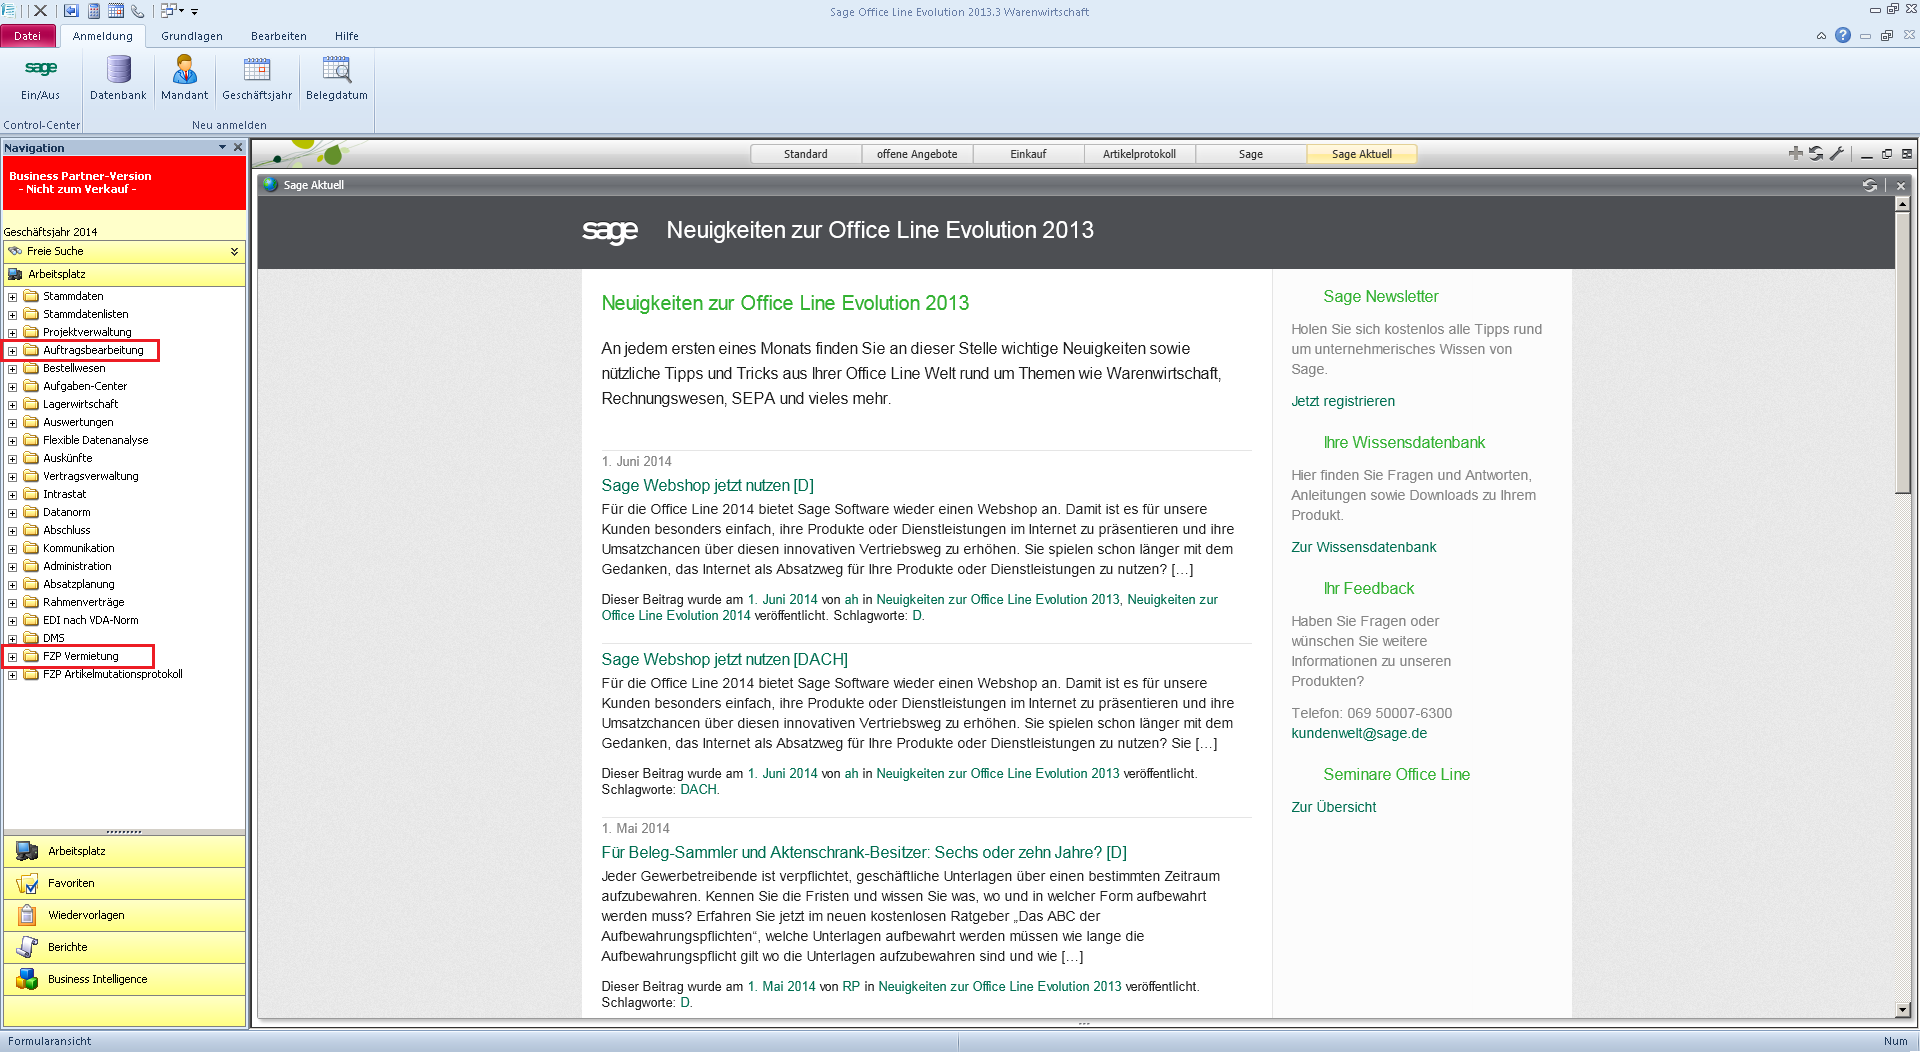
\includegraphics[height=300pt, width=\textwidth]{ol2.PNG}
    \caption[Hauptansicht Sage Office Line]{\small{Hauptansicht Sage Office Line}}
\end{figure}

\begin{figure}[!ht]
    \centering
    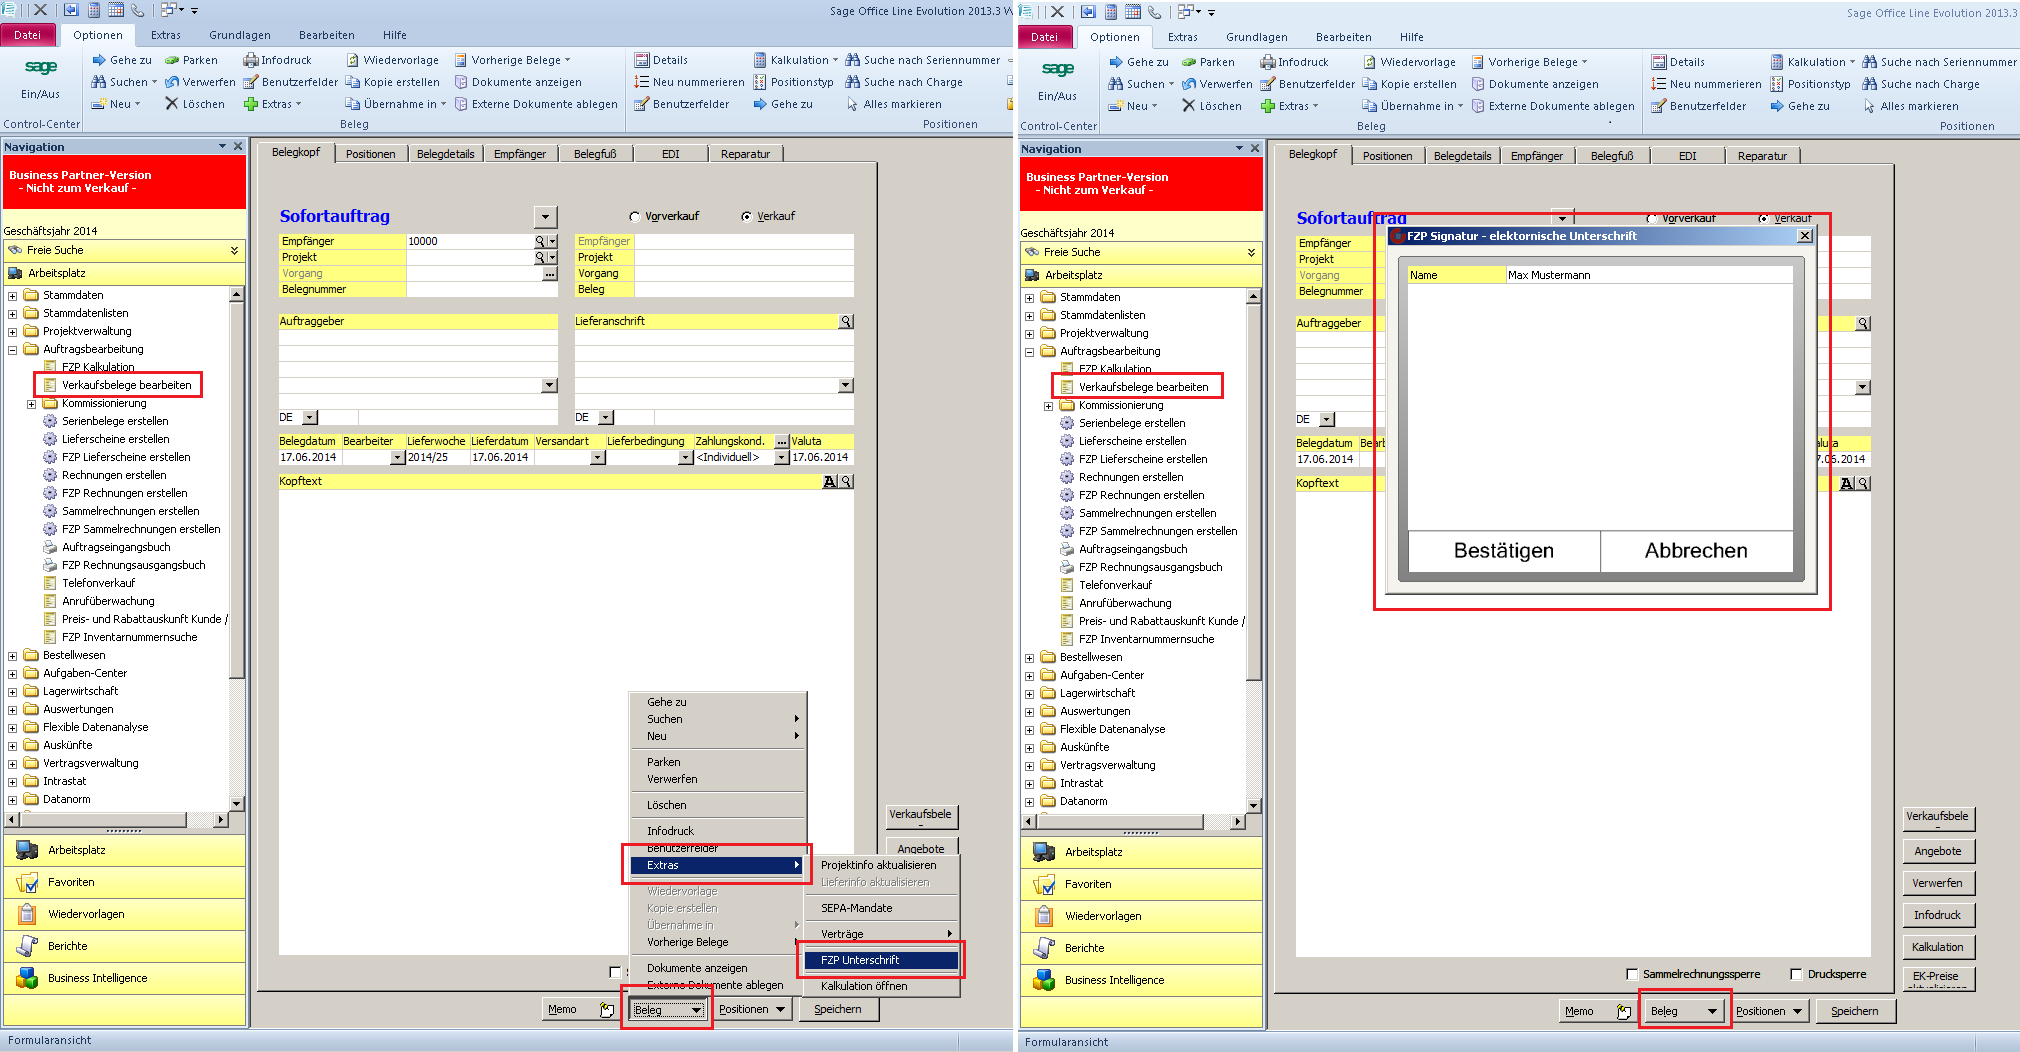
\includegraphics[height=250pt, width=\textwidth]{DigiSigVKBeleg3.png}
    \caption[Ablauf Erfassung digitale Signatur in Sage Office Line (Verkauf)]{\small{Ablauf Erfassung digitale Signatur im Bereich Verkauf in Sage Office Line}}
\end{figure}

\begin{figure}[!ht]
    \centering
    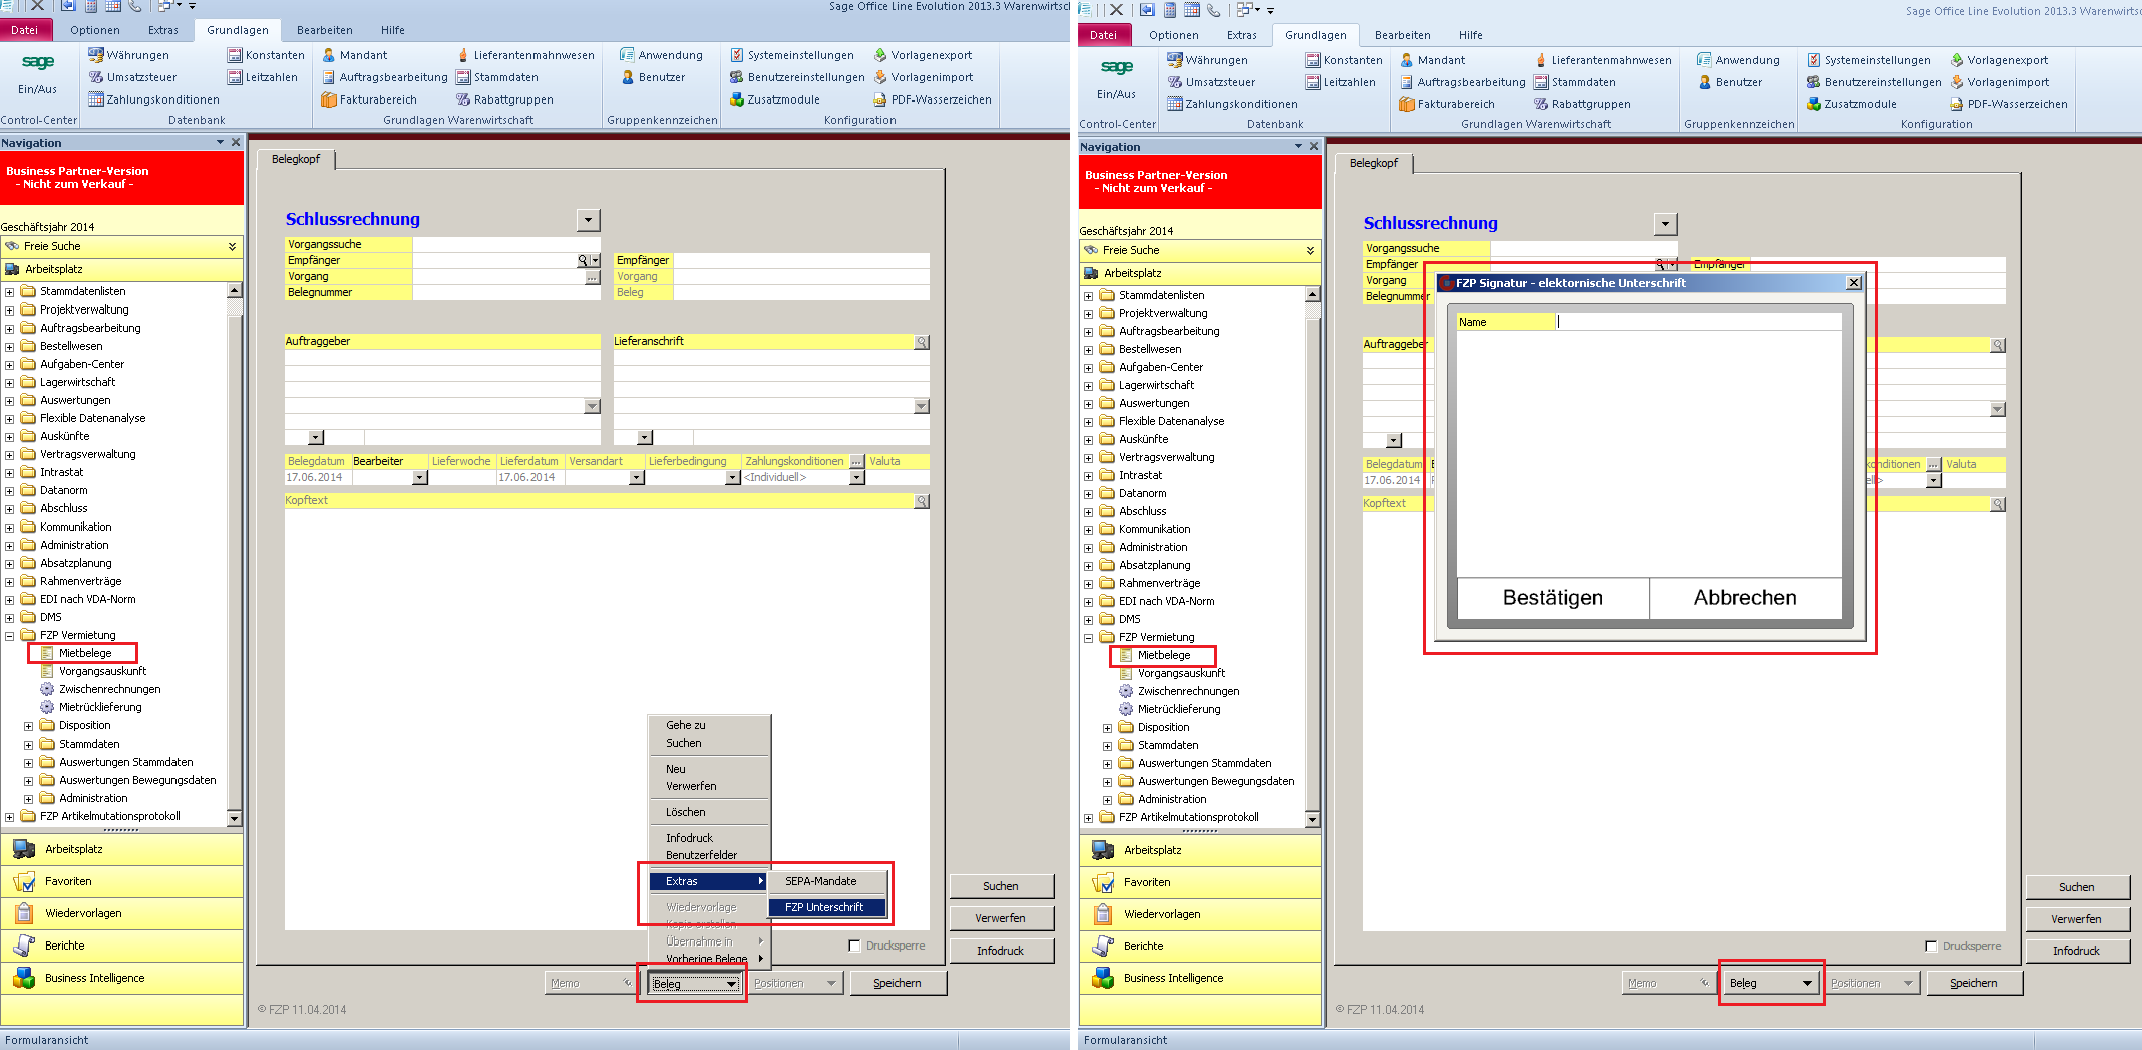
\includegraphics[height=250pt, width=\textwidth]{DigiSigVMBeleg3.png}
    \caption[Ablauf Erfassung digitale Signatur in Sage Office Line (Vermietung)]{\small{Ablauf Erfassung digitale Signatur im Bereich Vermietung in Sage Office Line}}
\end{figure}